\documentclass[10pt,a4paper]{article}
\usepackage[latin1]{inputenc}
\usepackage[spanish]{babel}
\usepackage{multicol}
\usepackage{amsmath}
\usepackage{amsfonts}
\usepackage{amssymb}
\usepackage{enumerate}
\usepackage{eurosym}
\usepackage{graphicx}
\usepackage{anysize}
\usepackage{colortbl}
\usepackage{hyperref}
\usepackage{lscape}
\usepackage{float}
\usepackage{longtable}
\usepackage{fancyhdr}
\pagestyle{fancy}
\marginsize{3cm}{2cm}{2cm}{2cm}
\setlength{\parskip}{1em}
\author{Jesus S�nchez-Oro Calvo}
\title{Documento de An�lisis Funcional}
\begin{document}

\thispagestyle{empty}
\begin{center}

\includegraphics[scale=1]{logoURJC.jpg} \\[1cm]
\textbf{\Huge Universidad Rey Juan Carlos}\\[0.5cm]
{\LARGE Escuela T�cnica Superior de Ingenier�a Inform�tica}\\[1.25cm]
{\Large Ingenier�a del Software II}\\[1.25cm]
{\LARGE \textbf{Pr�ctica Obligatoria}}\\[1.25cm]
{\LARGE \textit{Documento de Planificaci�n Inicial}}\\[2.5cm]
{\Large Radu Tom Vlad \\ David Rufo Valero \\ Jes�s S�nchez-Oro Calvo \\ Adri�n Santalla Romero de �vila }\\[1cm]
{\Large asantalla@siliconkernel.com}\\[2cm]
5� de Ingenier�a Inform�tica \\[1cm]
\today

\end{center}

\newpage
\fancyhead[LO,LE]{Ingenier�a del Software II}
\fancyhead[RO,RE]{Planificaci�n Inicial}
%\fancyfoot[LO,LE]{\thepage}
\tableofcontents

\newpage

\section{Necesidad del nuevo sistema y alcance del mismo}
El nuevo portal de Correos ha sido solicitado mediante un pliego de condiciones por la propia empresa solicitante, compuesto por dos partes bien diferenciadas:
	\begin{itemize}
	\item \textbf{An�lisis del sistema actual:} Es necesaria la realizaci�n de un an�lisis del sistema actual para obtener toda su funcionalidad, as� como para comprobar posibles fallos y mejoras a realizar.
	\item \textbf{Desarrollo de un nuevo portal:} Desarrollo del nuevo portal que va a sustituir al anterior, con los requisitos capturados.
	\end{itemize}
El alcance del sistema abarca ambos objetivos, obteniendo como principal producto final el nuevo portal de Correos.

\newpage

\section{Objetivos}
Los objetivos generales del actual desarrollo son los siguientes:
	\begin{itemize}
	\item \textbf{An�lisis de la funcionalidad disponible en el sistema actual:} Se llevar� a cabo realizando pruebas sobre todas las opciones disponibles en el portal actual, de manera que recorramos todas las funcionalidades de las que debe disponer el portal.
	\item \textbf{Comprobaci�n del sistema actual:} Se llevar� a cabo poniendo a prueba cada una de las funcionalidades del sistema actual para encontrar posibles defectos que deben ser corregidos
	\item \textbf{Determinaci�n de los elementos nuevos y modificaciones:} Se llevar� a cabo mediante la proposici�n de nuevas funcionalidades necesarias para el portal, as� como la modificaci�n de las funcionalidades anteriores para obtener una mejor respuesta.
	\item \textbf{Estudio previo del sistema:} Realizaci�n de un estudio previo donde se resumir� cual es el producto buscado en el desarrollo, as� como los requisitos generales.
	\item \textbf{An�lisis del sistema:} Realizaci�n de un an�lisis exhaustivo del nuevo sistema, donde aparezcan refinados todos los requisitos y dem�s necesidades del an�lisis.
	\item \textbf{Dise�o del sistema: }Realizaci�n de un dise�o del sistema de manera que quede listo para una posterior implementaci�n del mismo.
	\item \textbf{Prototipo:} Desarrollo de una serie de prototipos visuales donde pueda verse reflejado el estado final del sistema, as� como los datos que se van a mover a trav�s del mismo, representados a trav�s de un Cuaderno de Cargas.
	\end{itemize}
	
\newpage	
	
\section{Plan de Trabajo}
El plan de trabajo inicial establecido es el siguiente:
	\begin{figure}[H]
	\begin{center}
	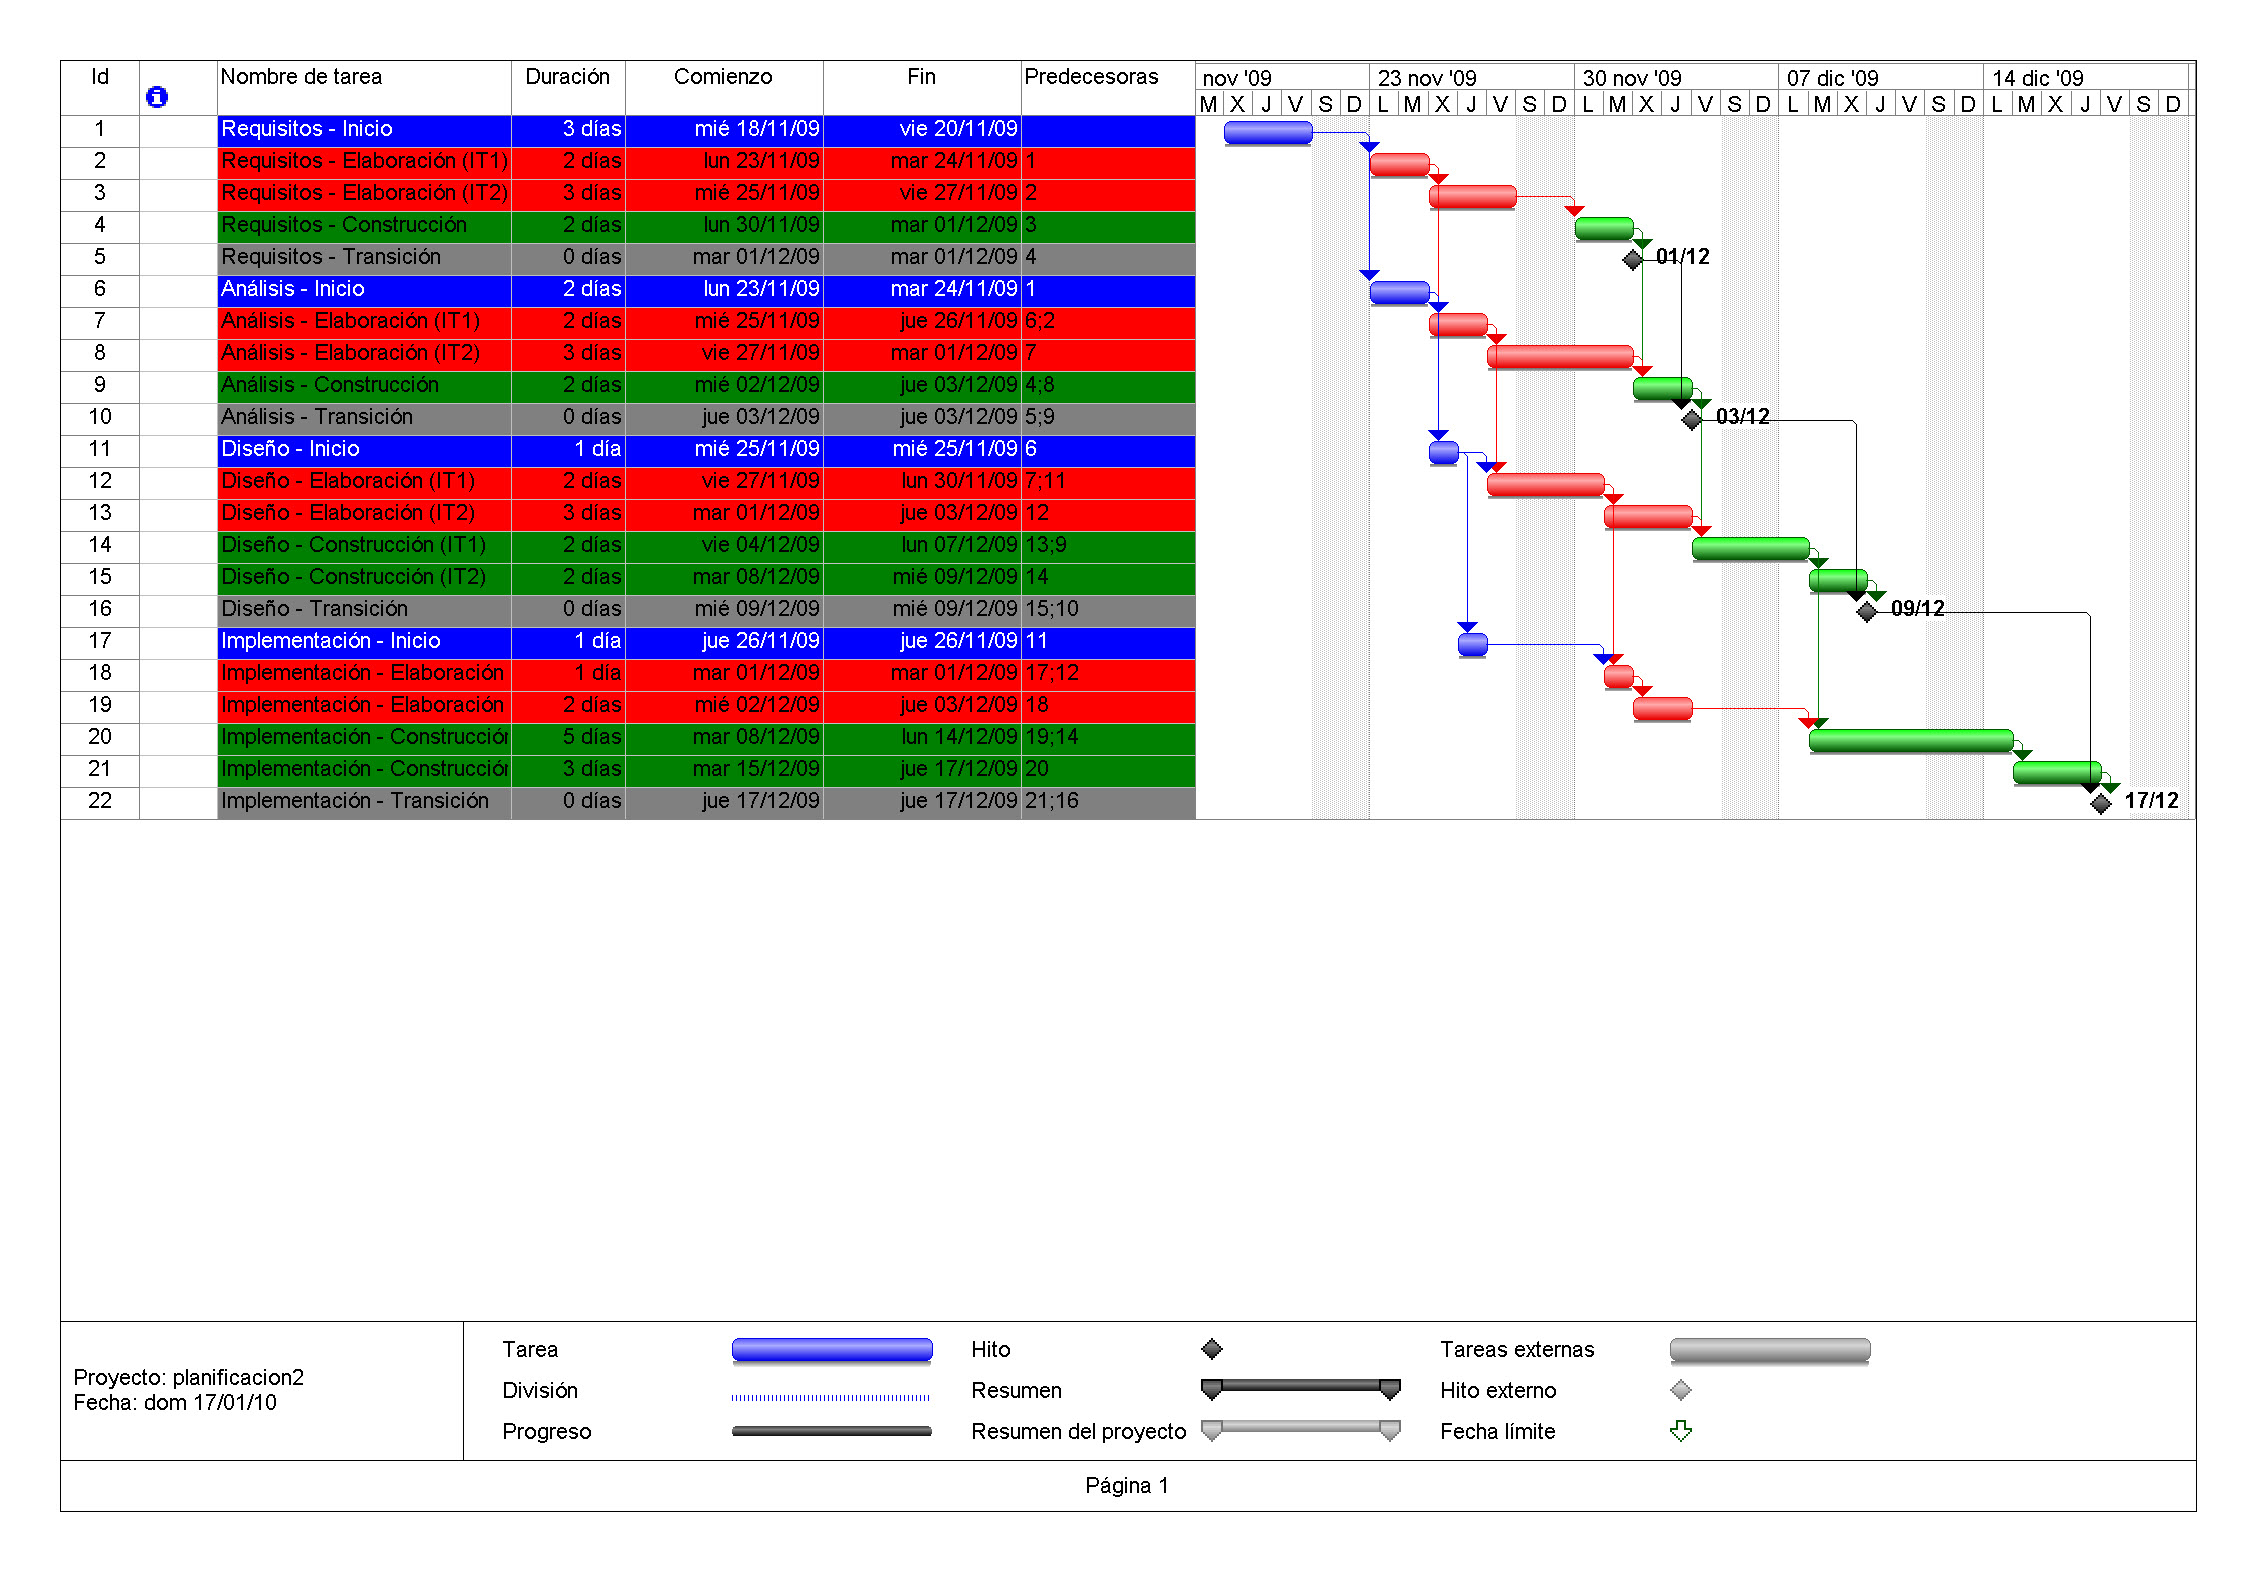
\includegraphics[scale=0.5]{planIni.jpg}
	\caption{Planificaci�n Inicial del Sistema}
	\end{center}
	\end{figure}
En esta planificaci�n, podemos ver resaltado en color azul las fase de Inicio con sus diferentes flujos de trabajo. El flujo de trabajo de requisitos es el m�s largo, debido a que ser� la captura de requisitos la que lleve m�s tiempo en esta fase de inicio. Del resto de fases no es necesario destacar ninguna.

\end{document}







